\documentclass{article}
\usepackage{graphicx}
\usepackage{color}
\usepackage{amsmath}
\usepackage{amssymb}
\usepackage{amsthm}
\usepackage{url}
%\usepackage{hyperref}
\usepackage[nottoc,numbib,notlof]{tocbibind}

% For Milnor's Lobachevsy function $\ML$ 
\usepackage[OT2,T1]{fontenc} 
\newcommand{\ML}{\mbox{\fontencoding{OT2}\fontfamily{wncyr}\fontseries{m}\fontshape{n}\selectfont L}} 

\usepackage[a4paper]{geometry}
\usepackage{fancyhdr}
\pagestyle{fancyplain}
\setlength{\parindent}{0pt}
\setlength{\parskip}{1ex}
\graphicspath{{image/}}

\newtheorem{definition}{Definition}
\newtheorem{proposition}{Proposition}

\title{Discrete differential geometry of surfaces. Variational principles, algorithms, and implementation}
\author{Stefan Sechelmann}

\begin{document}

\maketitle
\newpage

\tableofcontents
\newpage
\listoffigures

\newpage

\section{Introduction}
\section{Discrete Uniformization}

\subsection{Discrete conformal equivalence}

\begin{definition}
	Two Euclidean triangulations $T$ and $\tilde{T}$ are \emph{discretely conformally equivalent} if there is a map $u:V \to \mathbb{R}$ such that for any edge $ij$ it is
	\[l_{ij}=e^{u_i+u_j}\tilde{l}_{ij}\]
where $l_{ij}$ is the length of the edge $ij$.
\end{definition}

\begin{definition}
	A \emph{discrete flat metric} is a map $l:E\to\mathbb{R_+}$ such that triangle inequalities are satisfied and angle sums around each inner vertex are equal to $2\pi$. 
\end{definition}


\subsection{Variational principles for discrete metrics in $\mathbb{E}^2$, $\mathbb{H}^2$, and $\mathbb{S}^2$ }
Construction of discrete flat metrics. A discrete Euclidean flat metric is the minimizer of a convex functional.
\begin{eqnarray}
\lambda_{ij} &:=& 2\log l_{ij}\\
\tilde\lambda_{ij} &:=& \lambda_{ij}+u_i+u_j\\
f_{Euc}(u_i, u_j, u_k) &:=& \alpha_i \tilde \lambda_{jk} + \alpha_j \tilde \lambda_{ki} + \alpha_k \tilde \lambda_{ij} + 2\left(\ML(\alpha_i) + \ML(\alpha_j) + \ML(\alpha_k)\right)
\end{eqnarray}

\begin{definition}
\begin{eqnarray}
	E_{Euc}(u) &:=& \sum_{ijk\in F}\left(f_{Euc}(u_i, u_j, u_k) - \frac{\pi}{2}\left(\tilde \lambda_{jk} + \tilde \lambda_{ki} + \tilde \lambda_{ij}\right)\right) + \sum_{i\in V} \Theta_i u_i
\end{eqnarray}
\end{definition}

 This definition and the derivatives can be found in \cite{Bobenko2010}

For the hyperbolic case $\lambda$ and $\tilde\lambda$ are defined as before. Further define
\begin{eqnarray}
	\beta_i &:=& \frac{1}{2} \left(\pi + \alpha_i - \alpha_j - \alpha_k \right)\\
	\beta_j &:=& \frac{1}{2} \left(\pi - \alpha_i + \alpha_j - \alpha_k \right)\\
	\beta_k &:=& \frac{1}{2} \left(\pi - \alpha_i - \alpha_j + \alpha_k \right)\\
	f_{Hyp}(u_i, u_j, u_k) &:=&\beta_i \tilde \lambda_{jk} + \beta_j \tilde \lambda_{ki} + \beta_k \tilde \lambda_{ij}\\ 		
				&&+\ML(\alpha_i) + \ML(\alpha_j) + \ML(\alpha_k) + \ML(\beta_i) + \ML(\beta_j) + \ML(\beta_k)\\
				&&+\ML\left(\frac{1}{2} (\pi - \alpha_i - \alpha_j - \alpha_k)\right)
\end{eqnarray}

\begin{definition}
\begin{eqnarray}
	E_{Hyp}(u) &:=& \sum_{ijk\in F}\left(f_{Hyp}(u_i, u_j, u_k) - \frac{\pi}{2}\left(\tilde \lambda_{jk} + \tilde \lambda_{ki} + \tilde \lambda_{ij}\right)\right) + \sum_{i\in V} \Theta_i u_i
\end{eqnarray}
\end{definition}

\subsection{Realization}


\section{Uniformization of surfaces of higher genus}
Triangulated surfaces of genus $g\geq 2$ without boundary can be equipped with a discretely conformally equivalent flat hyperbolic metric \cite{Bobenko2010}. By flat hyperbolic metric we mean that the edge length are hyperbolic and for any vertex the angle sum is $2\pi$. To realize this metric in the hyperbolic plane e.g. in the Poicar\'e disk model one has to introduce cuts along a basis of the homotopy. This creates a simply connected domain in $\mathbb H^2$. Matching cut paths are realated by a hyperbolic motion i.e. the M\"obius transformations that leave the unit disk invariant (Figure~\ref{fig:axes_of_motion}).

\subsection{The cut-graph and fuchsian groups}
\emph{Want so say here: the number of transformations generated by the mapping of corresponding edges equals the number of path segments in the homotopy-cut-graph. They generate a fuchsian group with \#vertices relations}

\begin{proposition}
	
\end{proposition}

\begin{figure}
\centering
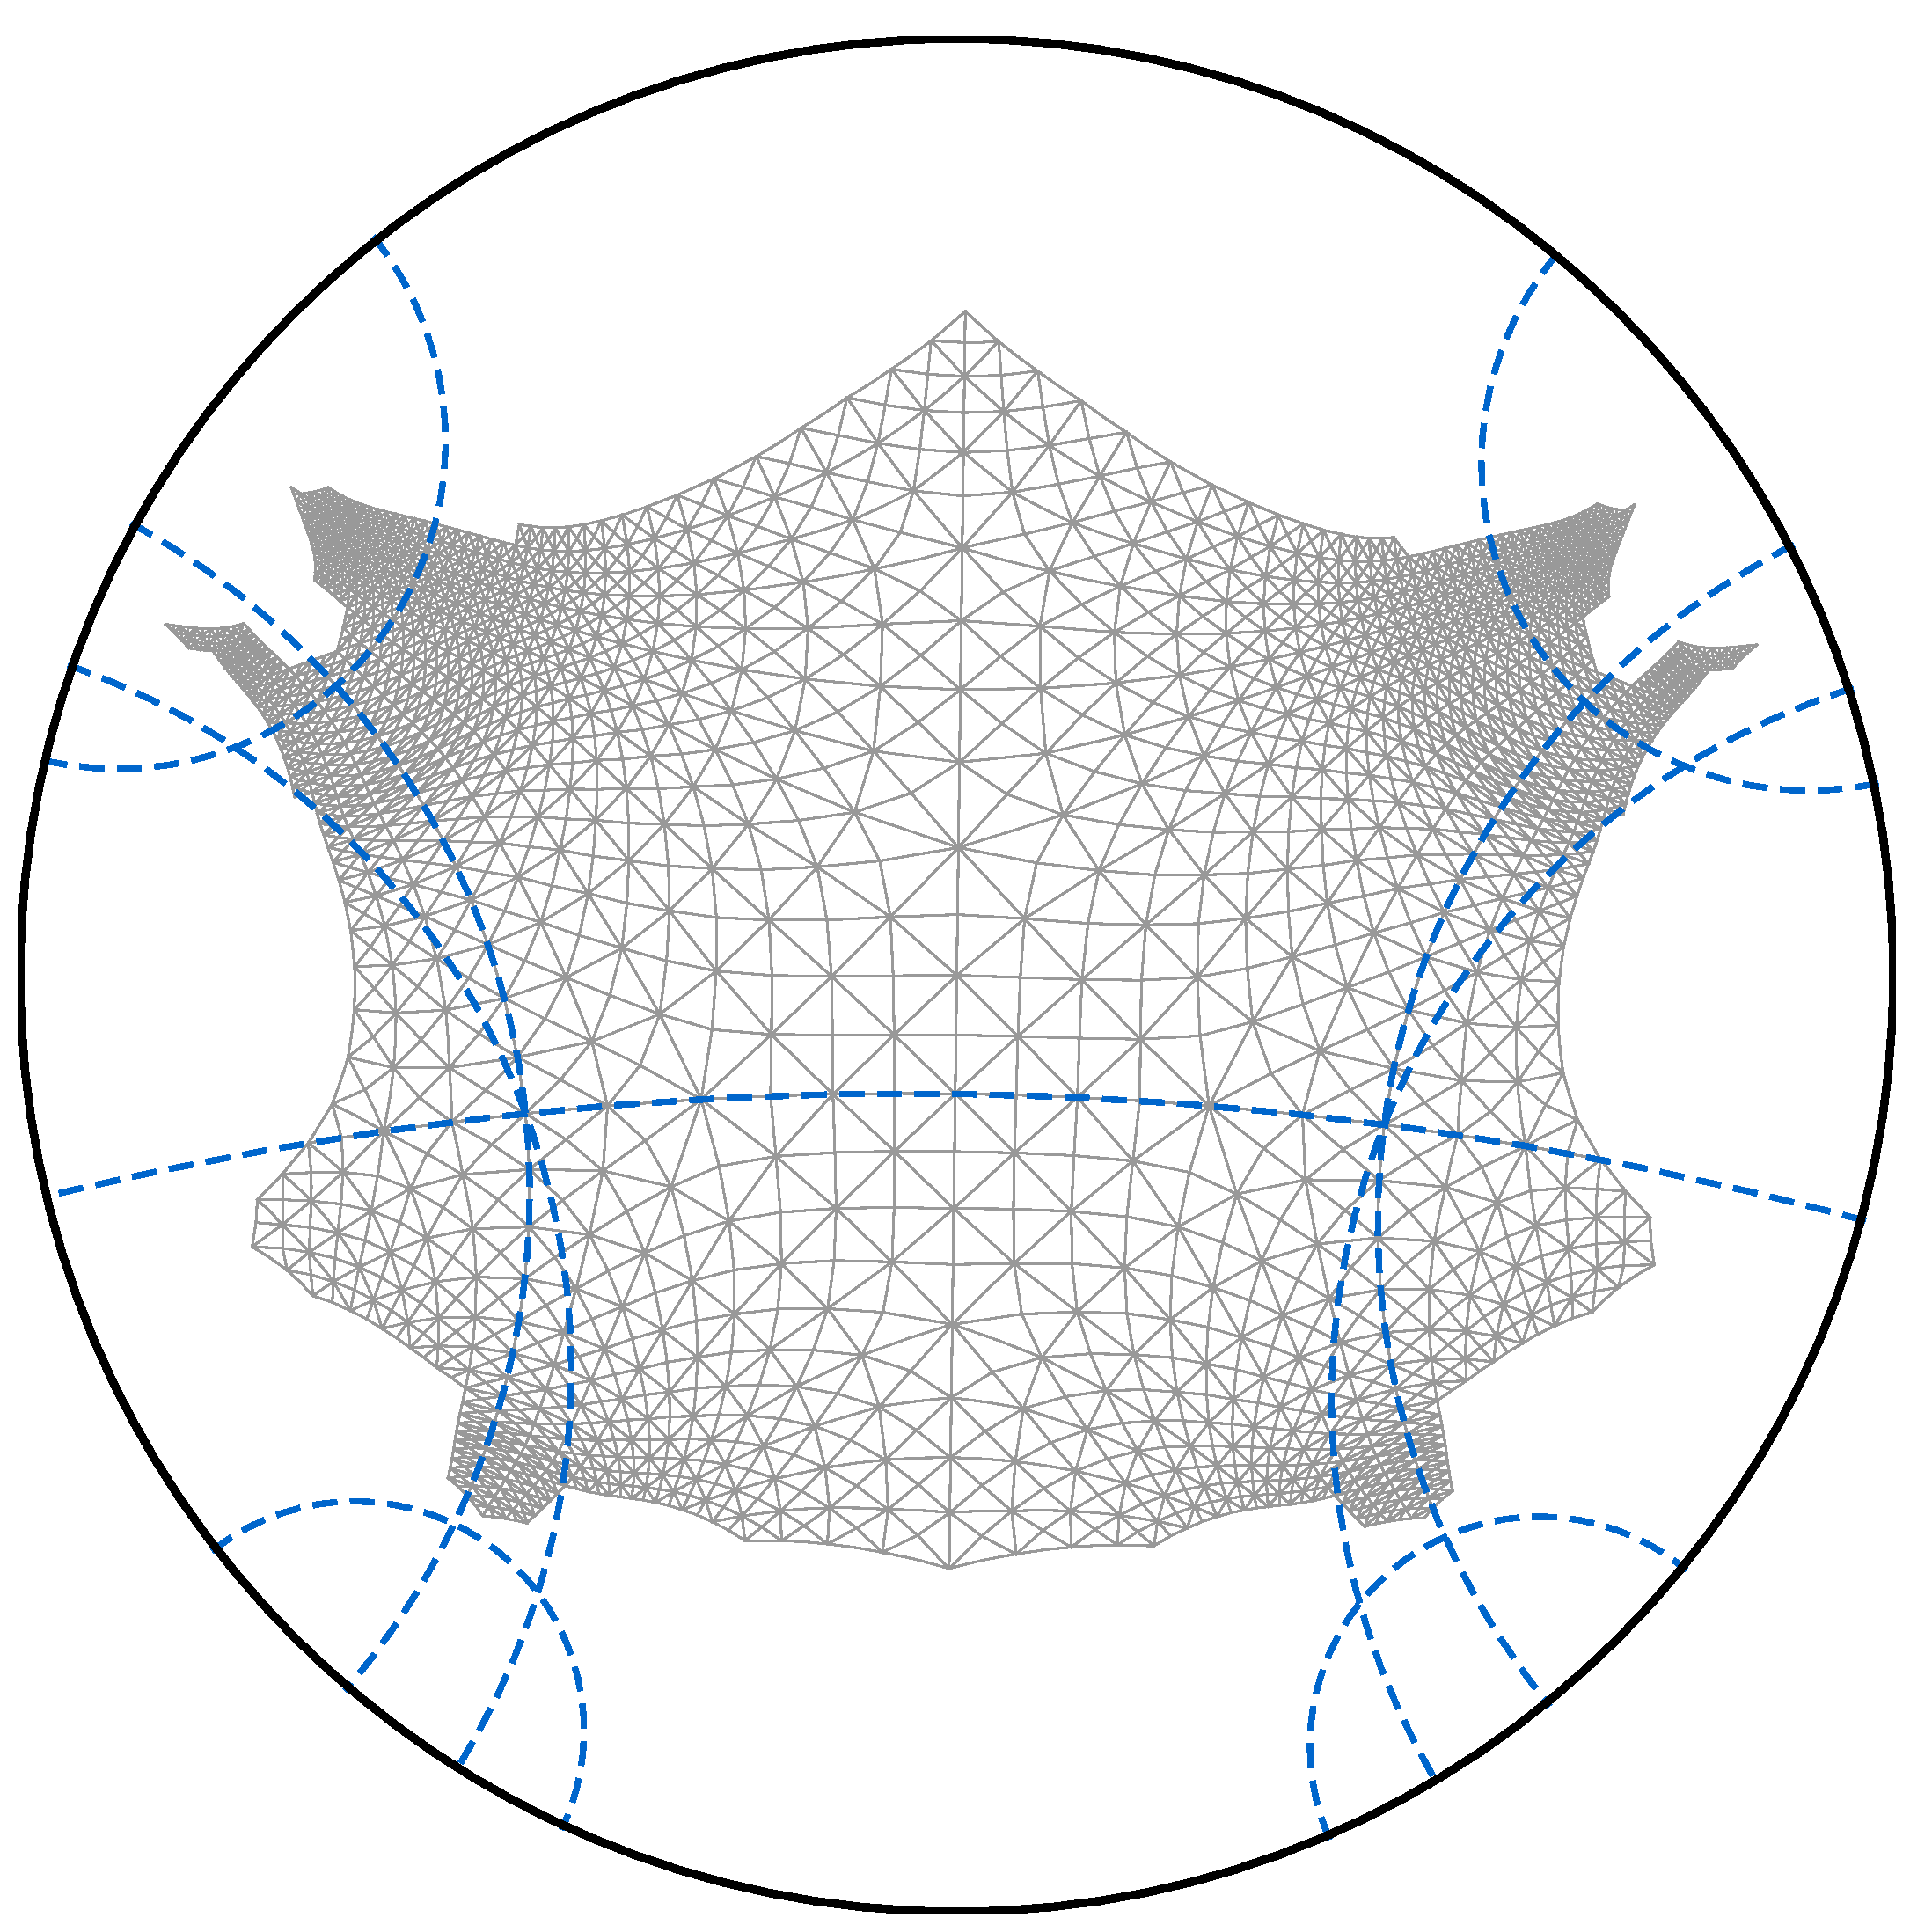
\includegraphics[width=0.4\linewidth]{cutCuttedBrezel01}
\caption{Hyperbolic flat metric on a genus $2$ surface and the axes of the associated hyperbolic motions.}
\label{fig:axes_of_motion}
\end{figure}

\subsection{Minimal presentation}

\section{Canonical fundamental domains of fuchsian groups}
\subsection{Separated handles}
\subsection{Opposite sides identified}

\section{Uniformization of tori}
\subsection{Elliptic Functions}
\subsection{The modul space}
\subsection{Numerical convergence analysis}

\section{Uniformization of hyperelliptic surfaces}
\subsection{Construction}
Any hyperelliptic Riemann surface can be expressed as an algebraic curve of the form
\[ \mu^2 = \prod_{i=1}^n(\lambda-\lambda_i)^2 \quad\quad n\geq3,\quad \lambda_i\neq \lambda_j \forall i\neq j.\]
Here $\lambda_i$ are the branch points of the doubly covered Riemann sphere.

\subsection{Weierstrass points on hyperelliptic surfaces}
A hyperelliptic surface comes together with a holomorphic involution $h$ called the hyperelliptic involution. The branch points are fixed points under this transformation. For a hyperelliptic algebraic curve it is $h(\mu, \lambda)=(-\mu, \lambda)$

\subsection{Canonical domains}

\section{Discrete quasi-isothermic parametrizations}
The notion of quasi-conformal parameterizations


\subsection{Discrete quasi-isothermic parameterizations}


\subsection{Boundary value problem}
\subsection{Variational principle for S-isothermic surfaces}
\subsection{A discrete ellipsoid and its dual surface}

\bibliographystyle{alpha}
\bibliography{Thesis}

\end{document}





































 